%%%%%%%%%%%%%%%%%%%%%%%%%%%%%%%%%%%%%%%%%%%%
% Chapitre 11
%%%%%%%%%%%%%%%%%%%%%%%%%%%%%%%%%%%%%%%%%%%%

\chapter{Contributions aux neurosciences}
\label{Chapter11}



% \minitoc

%----------------------------------------------------------------------------------------

\section{Sur la base de patients atteints de NMO}

\subsection{Résultats des méthodes linéaires}



% Fig. \ref{resNMO_1} shows the results obtained by the two scalar-based methods (\textit{GLM-FA} and \textit{GLM-MD}) and the Euclidean tensor-based method (\textit{GLM-DT})
% for the comparison between 34 NMO patients and 22 healthy subjects. 
% 
% The methods \textit{GLM-MD} and \textit{GLM-DT} present very similar results. 
% This observation is confirmed with the Dice coefficient always superior to $0.7$ for a wide range of thresholds (Fig. \ref{dice}).
% The main difference between the two methods concerns the putamen, which is a structure that has already been reported as involved in NMO~\cite{Zhao2012}
% and which is only detected by the  \textit{GLM-DT} and not by the \textit{GLM-MD}.
% The \textit{GLM-FA} method has a significantly different behavior as compared to  \textit{GLM-MD} and \textit{GLM-DT} (Fig. \ref{dice}).
% The most prominent difference  is that \textit{GLM-FA} does not detect alterations in the body of the corpus callosum and in the
% occipital lobe, which are structures that have also already been reported as involved in NMO~\cite{Yu2008,Rueda2012,Zhao2012}.
% 
% Finally, the major difference between the three methods concerns the statistical threshold requires to detect the 5\% of the most significant voxels within the white matter.
% The corresponding $p$-value thresholds are $p_{GLM-FA}=0.02$, $p_{GLM-MD}=0.04$ and $p_{GLM-DT}=0.002$.
% Consequently, \textit{GLM-DT} clearly outperforms the two other methods in terms of statistical power. Notice that for a $p$-value threshold of $0.002$,
% neither  \textit{GLM-FA}  nor  \textit{GLM-MD}  can detect any change. This gain in statistical power is explained by the fact that \textit{GLM-DT} relies on six times more data samples than the scalar-based methods.


\begin{figure*}[ht]
    \centering
    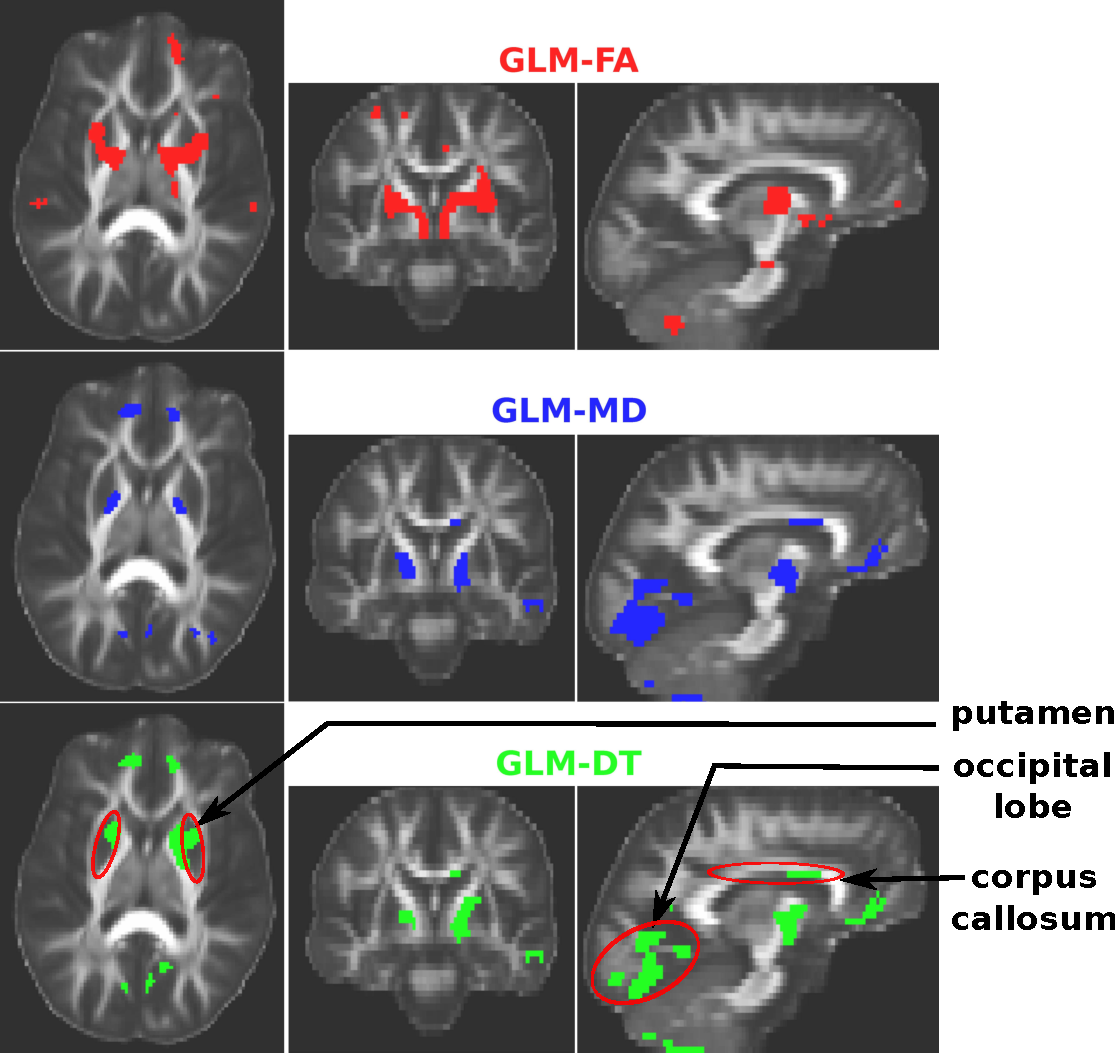
\includegraphics[width=0.9\textwidth]{Images/res_NMO_scalar_vs_tensor_annotations.pdf}
    \caption{\label{fig:nmo_1} Comparaison entre les méthodes basées sur les indices scalaires (\textit{GLM-FA} and \textit{GLM-MD}) 
    et la méthode basée sur les tenseurs avec une métrique Euclidienne (\textit{GLM-DT}).
    Les cartes statistiques sont seuillées de telle façon que seuls 5\% des voxels les plus significatifs dans le masque de la substance blanche sont retenus.
    La méthode des composantes connexes élimine les agrégats de taille inférieure à $N_c=10$ voxels.}
\end{figure*}

\subsection{Résultats des deux variétés géométriques}


\begin{figure*}[ht]
    \centering
    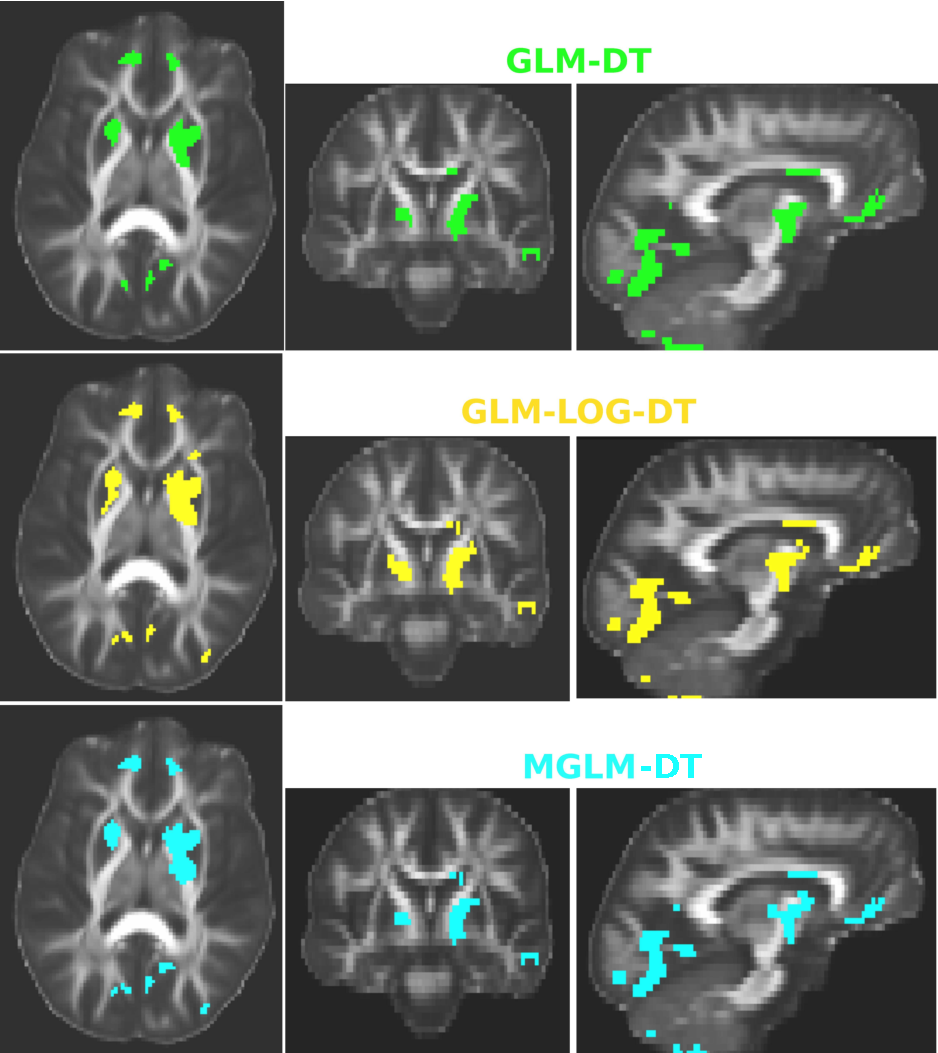
\includegraphics[width=0.8\textwidth]{Images/res_NMO_manifolds_annotations.pdf}
    \caption{\label{fig:nmo_2} Influence sur les méthodes basées tenseur de la métrique utilisée pour la comparaison de groupe entre les patients atteints de la NMO et les sujets contrôles.
    Les cartes statistiques sont seuillées de telle façon que seuls 5\% des voxels les plus significatifs dans le masque de la substance blanche sont retenus.
    La méthode des composantes connexes élimine les agrégats de taille inférieure à $N_c=10$ voxels.}
\end{figure*}


\subsection{Caractérisation}
La méthode de caractérisation est appliquée sur les cartes de détection obtenues avec la méthode \textit{GLM-DT}.
Au préalable, ces cartes dites \og primaires \fg sont corrigées par un FDR avec une seuil de $p_{FDR}=0.05$
et un technique de composantes connexes termine d'éliminer les détections résiduelles en ne conservant que les agrégats de taille supérieure à $N_c=10$.
Cette caractérisation appliquée à la carte primaire de la comparaison de sujets NMO \textit{vs} sujets sains, 
conduit à détecter 19 agrégats localisés sur 8 régions anatomiques différentes.

Le \tabref{tab:caracterisation} présente la liste de tous ces agrégats avec comme information : 
\begin{itemize}
    \item la région anatomique où se situe l'agrégat avec en information supplémentaire le côté,
    \item le (ou les) faisceau de la substance blanche touché,
    \item le signe du changement détecté :
    \begin{itemize}
        \item un \og $+$ \fg lorsqu'il s'agit d'un augmentation chez les sujets atteints par rapport aux sujets sains,
        \item un \og $-$ \fg dans le cas d'une diminution chez les sujets atteints par rapport aux sujets sains,
        \item une abbréviation \og n.s. \fg lorsque l'agrégat n'est pas significatif pour l'indice scalaire étudié.
    \end{itemize}
\end{itemize}



% Moreover the sign and the statistical significance ($p<0.05$) of the change for each scalar index (MD and FA) and each cluster are reported (see Table \ref{tab:characterisation2}).
% 
% The results show eight clusters classified as deleterious changes, four as favorable changes and seven as uncategorisable changes.
% 
% Five clusters in the occipital lobe are characterized by an augmentation of the mean diffusivity in the patient group as compared to the control group, 
% which may reflect a demyelination that is probably related to the visual disorders induced by the pathology.
% Similar signatures are observed for clusters located in the hippocampus and the corpus callosum.
% Two clusters, respectively in the parietal lobe and the frontal lobe 
% (cluster on the left inferior fronto-occipital tract and the genu of the corpus callosum) 
% present a radial diffusion augmentation and an axial diffusion diminution which can also be linked to a demyelination process.
% The four clusters that are categorized as favorable changes might be the consequences of compensation phenomena or therapeutic drugs effects.
% The remaining clusters belong to the uncategorisable group.
% 
% We are well aware that there are multiple others options to process this kind of classification.
% We choose this direct way to do because of the procedure user friendlyness, the computational efficiency 
% and the similar approach of the detection method (both based on the GLM with the same covariables).

\begin{table}[htbp]
\centering
\begin{tabular}{|D{3.5cm}|D{0.5cm}|D{4.5cm}|D{1.2cm}|D{1.2cm}|}
      \hline
      \multicolumn{2}{|c|}{\textbf{Localisation}} & \textbf{Faisceau impacté} & \textbf{MD} & \textbf{FA} \tabularnewline
      \hline
      \hline
      \multirow{5}{*}{Lobe occipital} & d. & optic radiation \\ faisceau long. inf. \\ corps calleux (splenium) & $+$ & $n.s.$ \tabularnewline
       \cline{2-5}
       & g. & optic radiation \\ corps calleux (splenium) & $+$ & $n.s.$ \tabularnewline
       \cline{2-5}
       & g. & optic radiation \\ inf. long. fasciculus \ corps calleux (splenium) & $+$ & $n.s.$ \tabularnewline
       \cline{2-5}
       & d. & inf. fronto-occipital fasciculus & $+$ & $n.s.$ \tabularnewline
       \cline{2-5}
       & d. & \cellcolor[gray]{0.9} & $n.s.$ & $n.s.$ \tabularnewline
      \hline
      Hippocampe & g. & \cellcolor[gray]{0.9} & $+$ & $n.s.$ \tabularnewline
      \hline
      Corps calleux & d. & corps calleux (body) & $+$ & $n.s.$ \tabularnewline
      \hline
      Lobe pariétal & d. & faisceau long. sup. & $+$ & $-$ \tabularnewline
      \hline
      \multirow{3}{*}{Lobe frontal} & g. & corps calleux (genu) \\ inf. fronto-occipital & $-$ & $-$ \tabularnewline
       \cline{2-5}
       & d. & inf. fronto-occipital & $n.s.$ & $n.s.$ \tabularnewline
       \cline{2-5}
       & g. & corps calleux (genu) & $-$ & $+$ \tabularnewline
      \hline
      \multirow{2}{*}{Capsule interne} & d. & inf. fronto-occipital\\ dentate-rubro-thalamo cortical & $n.s.$ & $n.s.$ \tabularnewline
       \cline{2-5}
       & d. & faisceau cortico-spinal & $-$ & $n.s.$ \tabularnewline
      \hline
      \multirow{2}{*}{Lobe temporal} & d. & faisceau arcqué & $n.s.$ & $n.s.$ \tabularnewline
       \cline{2-5}
       & d. & faisceau long. inf. & $-$ & $n.s.$ \tabularnewline
      \hline
      \multirow{4}{*}{Cervelet} & d. & \cellcolor[gray]{0.9} & $-$ & $n.s.$ \tabularnewline
       \cline{2-5}
       & g. & \cellcolor[gray]{0.9} & $n.s.$ & $n.s.$ \tabularnewline
       \cline{2-5}
       & g. & \cellcolor[gray]{0.9} & $n.s.$ & $n.s.$ \tabularnewline
       \cline{2-5}
       & d. & \cellcolor[gray]{0.9} & $n.s.$ & $n.s.$ \tabularnewline
      \hline
  \end{tabular}
  \caption{\label{tab:caracterisation} Résultats ($p_\text{corrigées}<0.05$) de la caractérisation pour la méthode \textit{GLM-DT} (seuil statistique $p_{FDR}=0.05$ et seuil $N_c=10$).
  (Légende: $+=$ augmentation significative, $-=$ diminution significative, $n.s.=$ non significatif, d. $=$ droite, l. $=$ gauche, inf. $=$ inférieur, sup. $=$ supérieur, long. $=$ longitudinale)}
\end{table}

\section{Sur la base de patients atteints de DLB}
\subsection{Comparaison de patients au stade prodomal avec des témoins}
\subsection{Étude sur les hallucinations dans le maladie à corps de Lewy}


